\documentclass[a4paper,12pt]{article}

\usepackage{abakos}
\usepackage{abntex2cite}
\usepackage{placeins}
\usepackage{framed}

%%%%%%%%%%%%%%%%%%%%%%%%%%%
%Capa da revista
%%%%%%%%%%%%%%%%%%%%%%%%%%

%\setcounter{page}{80} %iniciar contador de pagina de valor especificado, quando o artigo for alocado a uma edição
\newcommand{\monog}{Roteamento Dinâmico de Consultas SQL Baseado em Metadados de Tabelas Apache Iceberg}
\newcommand{\monogES}{Dynamic SQL Query Routing Based on Apache Iceberg Table Metadata}
\newcommand{\origem}{Brasil}
\newcommand{\editorial}{} % p. xx-xx — páginas inicial-final do artigo
% \newcommand{\lcc}{\scriptsize{Licença Creative Commons Attribution-NonCommercial-NoDerivs 3.0 Unported}}

%%%%%%%%%%%%%%%%%INFORMAÇÕES SOBRE AUTORES %%%%%%%%%%%%%%%%%%%%%%%%%%%%%%%
\newcommand{\AutorA}{Aristides Henrique Gonçalves da Cruz}
\newcommand{\funcaoA}{Engenheiro de Dados}
\newcommand{\cursA}{Sistemas de Informação}
\newcommand{\emailA}{arihenriquedev@hotmail.com}

%Comentar essas 4 linhas, caso o TCC seja desenvolvido individualmente
% \newcommand{\AutorB}{Nome do Segundo Autor}
% \newcommand{\funcaoB}{}
% \newcommand{\cursB}{Afiliação do autor 2}
% \newcommand{\emailB}{autor2@email.edu.br}

\newcommand{\AutorC}{Gustavo Luís Soares}
\newcommand{\funcaoC}{Orientador}
\newcommand{\cursC}{Instituto de Ciências Exatas e de Informática da PUC Minas}
\newcommand{\emailC}{gsoares@pucminas.br}

\newcommand{\keyword}[1]{\textsf{#1}}
\newcommand{\fonte}[1]{\begin{center}\textbf{\footnotesize Fonte: #1}\end{center}}

\begin{document}

% %%%%%%%%%%%%%%%%%%%%%%%%%%%%%%%%%%
% %% Pagina de titulo
% %%%%%%%%%%%%%%%%%%%%%%%%%%%%%%%%%%

\begin{flushleft}
%\begin{minipage} [c][5cm][b]{16.5cm} % Cabeçalho da primeira página da revista
%
\includegraphics[scale=1.1]{figuras/pucmg.png} 
%\end{minipage}
\vspace{0cm} { %Rodapé das páginas da revista
\singlespacing \Large{\monog \symbolfootnote[1]{Trabalho de conclusão de curso, Sistemas de Informação, Unidade São Gabriel} \\ }
\normalsize{\monogES}
}
\end{flushleft}

\begin{flushright}
\singlespacing 
\normalsize{\AutorA \footnote{\funcaoA, \cursA, \origem -- \emailA }} \\

%Comentar essa linha, caso o TCC seja desenvolvido individualmente
% \normalsize{\AutorB \footnote{\funcaoB, \cursB, \origem -- \emailB }} \\

 \normalsize{\AutorC \footnote{\funcaoC, \cursC, \origem -- \emailC }} \\
\end{flushright}
\thispagestyle{empty}

% Inclusão do resumo
\begin{abstract}
    \noindent
    O crescimento do volume de dados em \textit{data lakes} tem impulsionado a necessidade de arquiteturas adaptativas que equilibrem custo e \textit{performance} na execução de consultas SQL. Este trabalho apresenta o \textit{DyraSQL}, um \textit{framework} para roteamento dinâmico de consultas SQL baseado em metadados de tabelas \textit{Apache Iceberg}, obtidos por meio do comando \textit{EXPLAIN (TYPE IO)} do \textit{Trino}. O sistema direciona automaticamente consultas para \textit{clusters} de processamento com capacidades distintas, classificados como \textit{small}, \textit{medium} e \textit{large}, a partir de um algoritmo de pontuação que combina volume de dados, complexidade da consulta e histórico de execuções. A metodologia envolve extração de metadados sobre volume efetivo e custos de I/O, análise sintática da consulta SQL e reaproveitamento de decisões em \textit{cache} temporal no PostgreSQL. O protótipo foi avaliado em ambiente local orquestrado por Docker Compose, com tabelas \textit{Apache Iceberg} geradas sobre armazenamento de objetos MinIO e catálogo REST, demonstrando que o sistema calcula \textit{scores} consistentes e classifica consultas nas faixas de capacidade definidas. Os resultados indicam que o roteamento baseado em metadados contribui para o uso mais eficiente de recursos de processamento, oferecendo um modelo adaptativo aplicável a \textit{clusters} \textit{Trino} locais e, em trabalhos futuros, a ambientes de nuvem.
    \\\textbf{\keyword{Palavras-chave: }} Consultas SQL. Trino. Apache Iceberg. Data lake. Trino Gateway.
    \end{abstract}


%%%%%%%%%%%%%%%%%%%%%%%%%%%%%%%%%%%%%%%%%%%%%%%%%%%%%%%%%
\newpage 

% Inclusão do abstract em inglês
\selectlanguage{english}
\begin{abstract}
\noindent
The growth of data volume in data lakes has increased the need for adaptive architectures that balance cost and performance in SQL query execution. This work presents DyraSQL, a framework for dynamic SQL query routing based on Apache Iceberg table metadata obtained through Trino's EXPLAIN (TYPE IO) command. The system automatically directs queries to processing clusters with distinct capacities, classified as small, medium, and large, using a scoring algorithm that combines data volume, query complexity, and execution history. The methodology extracts metadata about effective data volume and I/O costs, performs syntactic analysis of SQL queries, and reuses decisions through a temporal cache in PostgreSQL. The prototype was evaluated in a local Docker Compose environment, with generated Apache Iceberg tables on MinIO object storage and a REST catalog, showing that the system computes consistent scores and classifies queries into the defined capacity ranges. The results indicate that metadata-based routing contributes to more efficient use of processing resources, offering an adaptive model for local Trino clusters and, as future work, for cloud environments.
\\\textbf{\keyword{Keywords: }} SQL queries. Trino. Apache Iceberg. Data lake. Trino Gateway.
\end{abstract}
\selectlanguage{brazilian}


\newpage

\selectlanguage{brazilian}
 \onehalfspace  % espaçamento 1.5 entre linhas
 \setlength{\parindent}{1.25cm}

%%%%%%%%%%%%%%%%%%%%%%%%%%%%%%%%%%%%%%%%%%%%%%%%%
%% INICIO DO TEXTO
%%%%%%%%%%%%%%%%%%%%%%%%%%%%%%%%%%%%%%%%%%%%%%%%%

% Inclusão da introdução
\section{Introdução}
\label{sec:introducao}

O crescimento do volume de dados tem impulsionado a adoção de arquiteturas escaláveis para análise e tomada de decisão \cite{ibmbigdata}. Nesse contexto, o desafio não está apenas em armazenar grandes volumes de dados de forma eficiente, mas também em processá-los equilibrando custos e desempenho \cite{weintraub2024}. A arquitetura de \textit{data lakes} baseada em armazenamento de objetos oferece escalabilidade e custos reduzidos, sendo que a separação entre camadas de armazenamento e processamento permite utilização de recursos computacionais em modo \textit{on-demand} \cite{dremiodatalake,weintraub2024}.

Ferramentas como o \textit{Apache Iceberg} têm se destacado ao permitir a gestão eficiente de tabelas em \textit{data lakes}, oferecendo versionamento, \textit{schema evolution} e melhorias de consulta \cite{iceberg2024}. Mecanismos de execução distribuída, como o \textit{Trino}, viabilizam consultas de alta \textit{performance} sobre dados armazenados em sistemas de objetos, por meio de processamento distribuído entre múltiplos nós trabalhadores \cite{trinoconcepts}. No entanto, a escolha do ambiente de execução das consultas ainda tende a ser estática, sendo que sistemas tradicionais não adaptam automaticamente a infraestrutura de processamento às características específicas de cada consulta \cite{weintraub2024,xue2024}. Trabalhos recentes têm explorado roteamento baseado em modelos de custo aprendidos \cite{strausz2025} e elasticidade em tempo de execução para análise de dados em nuvem \cite{zhang2025}.

A pesquisa propõe o \textit{DyraSQL}, uma abordagem adaptativa para direcionamento de consultas SQL, considerando características previamente disponíveis nos metadados. A proposta consiste em analisar a complexidade das consultas e o volume efetivo de dados antes da execução e, a partir disso, direcioná-las para \textit{clusters} \textit{Trino} de capacidades distintas, classificados como \textit{small}, \textit{medium} e \textit{large}. Tal abordagem busca viabilizar uma utilização mais eficiente dos recursos disponíveis, equilibrando custo e \textit{performance}. Xue et al. (2024) demonstram a importância de execução adaptativa de consultas em ambientes de \textit{data lakehouse} \cite{xue2024}, reforçando a relevância desta pesquisa.

A capacidade de direcionar automaticamente consultas para o ambiente mais adequado resulta em melhor utilização de recursos computacionais e em redução de provisionamento excessivo para consultas leves. Este trabalho desenvolve o \textit{DyraSQL}, um mecanismo de decisão que utiliza informações de metadados para definir, de forma automática, o \textit{cluster} mais adequado para a execução de consultas SQL. Para alcançar este propósito, o trabalho mapeia os metadados disponíveis em tabelas \textit{Apache Iceberg}, identificando quais podem ser utilizados como indicadores de volume de dados, complexidade da consulta e custo esperado de execução. Estabelece regras de decisão para roteamento, definindo parâmetros que permitam classificar consultas nas três faixas de capacidade. Projeta e desenvolve um protótipo funcional do \textit{DyraSQL} em ambiente local, utilizando o \textit{Trino} como \textit{engine} de consultas, Docker Compose para orquestração, MinIO para armazenamento de objetos e PostgreSQL para \textit{cache} e histórico. Realiza experimentos controlados nesse ambiente, a fim de verificar a viabilidade técnica do \textit{DyraSQL} e coletar métricas de consistência dos \textit{scores}, latência do \textit{EXPLAIN (TYPE IO)} e comportamento do \textit{cache}. Compara o comportamento do roteamento dinâmico com a lógica estática de um único \textit{cluster}, avaliando a capacidade do algoritmo de diferenciar consultas leves, intermediárias e pesadas.

Este trabalho está organizado da forma apresentada. A Seção~\ref{sec:referencial-teorico} aborda o referencial teórico. A Seção~\ref{sec:revisao-bibliografica} apresenta a revisão bibliográfica. A Seção~\ref{sec:metodologia} detalha a metodologia. A Seção~\ref{sec:experimentos} apresenta os experimentos e resultados. A Seção~\ref{sec:consideracoes-finais} apresenta as considerações finais e trabalhos futuros.


% Inclusão do referencial teórico
\section{Referencial Teórico}
\label{sec:referencial-teorico}

Esta seção apresenta os conceitos fundamentais que embasam a pesquisa proposta, abordando arquiteturas de \textit{data lakes}, análise de dados em \textit{big data}, tecnologias de processamento distribuído e o roteamento de consultas utilizado no desenvolvimento do \textit{DyraSQL}. Os tópicos são organizados de forma a estabelecer o contexto teórico necessário para compreensão da solução proposta.

\subsection{Arquiteturas de \textit{Data Lake}}

\textit{Data lakes} representam repositórios centralizados que armazenam grandes volumes de dados em seu formato bruto, sem estruturação prévia, permitindo armazenamento escalável e flexível para diferentes tipos de análises \cite{dremiodatalake}. Diferentemente de \textit{data warehouses}, que organizam dados em esquemas estruturados pré-definidos, \textit{data lakes} mantêm dados em formato nativo, facilitando a ingestão de dados diversos e a exploração analítica posterior \cite{dremiodatalake}. Esta arquitetura é particularmente adequada para ambientes de \textit{big data}, nos quais o volume, variedade e velocidade dos dados tornam a estruturação prévia impraticável ou limitante \cite{ibmbigdata}.

A arquitetura de \textit{data lakes} baseada em armazenamento de objetos oferece escalabilidade e custos reduzidos de armazenamento, sendo que os dados são organizados em \textit{buckets} e objetos, permitindo acesso direto através de APIs \cite{dremiodatalake}. Esta abordagem elimina a necessidade de provisionamento prévio de capacidade, permitindo que organizações armazenem grandes volumes de dados de forma econômica \cite{ibmbigdata}. O \textit{DyraSQL} aproveita esta arquitetura para acessar metadados de tabelas \textit{Apache Iceberg} armazenadas em \textit{data lakes}, utilizando informações sobre volume e estrutura dos dados para tomada de decisões de roteamento. No protótipo local, o armazenamento de objetos é provido pelo MinIO, que expõe uma API compatível com sistemas de objetos utilizados em \textit{data lakes}.

\subsection{Análise de Dados em \textit{big data}}

A análise de dados em \textit{big data} envolve o processamento de volumes massivos de informações que excedem a capacidade de sistemas tradicionais de banco de dados, requerendo arquiteturas distribuídas e técnicas especializadas de processamento \cite{ibmbigdata}. Os desafios principais incluem o volume dos dados, a variedade de formatos e fontes, a velocidade de geração e a necessidade de extrair valor em tempo hábil para tomada de decisão \cite{ibmbigdata}. Sistemas de processamento distribuído, como Apache Spark e \textit{Trino}, viabilizam a análise de grandes volumes de dados através de paralelização e distribuição de carga de trabalho entre múltiplos nós computacionais \cite{apachespark2025,trinoconcepts}. O Apache Spark é um \textit{engine} unificado de análise para processamento de dados em larga escala, fornecendo APIs de alto nível e um \textit{engine} que suporta grafos de execução gerais \cite{apachespark2025}.

A eficiência na análise de \textit{big data} depende da escolha adequada da arquitetura de processamento, sendo que consultas leves podem ser executadas em \textit{clusters} menores, enquanto consultas complexas requerem infraestrutura com maior capacidade computacional \cite{ibmbigdata}. O \textit{DyraSQL} aborda este desafio através de roteamento dinâmico que direciona consultas para o \textit{cluster} mais adequado baseado em características dos dados e complexidade das operações, melhorando o custo-benefício do processamento.

\subsection{\textit{Trino}}

O \textit{Trino} é um \textit{engine} de consultas SQL distribuído projetado para consultar grandes volumes de dados armazenados em diversos sistemas, incluindo \textit{data lakes} baseados em armazenamento de objetos \cite{trinoconcepts}. A arquitetura do \textit{Trino} é baseada em um modelo de coordenação distribuída, sendo que um nó coordenador recebe consultas SQL e coordena a execução entre múltiplos nós trabalhadores (\textit{workers}), cada um processando uma porção dos dados em paralelo \cite{trinoconcepts}. Esta arquitetura permite escalabilidade horizontal através da adição de nós trabalhadores, aumentando a capacidade de processamento conforme a demanda cresce \cite{trinoconcepts}.

O \textit{Trino} suporta conectores para diversos sistemas de armazenamento, incluindo \textit{Apache Iceberg}, permitindo consultas SQL unificadas sobre dados armazenados em diferentes formatos e localizações \cite{trinoconcepts}. O \textit{DyraSQL} utiliza o \textit{Trino} como \textit{engine} de consultas, aproveitando sua capacidade de processamento distribuído e o suporte nativo a tabelas \textit{Apache Iceberg}. A integração com \textit{Trino Gateway} permite roteamento de consultas para diferentes \textit{clusters} de execução baseado em análise prévia de metadados \cite{trinogateway}. No ambiente experimental, o conector \textit{Iceberg} é configurado com catálogo REST, de modo que múltiplos \textit{clusters} compartilhem o mesmo catálogo e o mesmo \textit{warehouse} de objetos.

\subsection{Catálogo de Metadados}

Sistemas de consulta sobre \textit{data lakes} dependem de um catálogo que descreva esquemas, localização dos dados e estatísticas das tabelas, permitindo que o \textit{engine} descubra e acesse os dados sem conhecer a estrutura física dos arquivos \cite{apachehive2025}. O Apache Hive popularizou o \textit{Hive Metastore} como catálogo compartilhado entre ferramentas de análise \cite{apachehive2025}. O \textit{Apache Iceberg} admite diferentes implementações de catálogo, incluindo o \textit{Hive Metastore} e o catálogo REST, que expõe uma API HTTP para operações de metadados \cite{iceberg2024}.

O \textit{DyraSQL} não depende de um provedor específico de catálogo. O protótipo local utiliza o catálogo REST do \textit{Apache Iceberg} compartilhado pelos \textit{clusters} \textit{Trino}, garantindo consistência de metadados independentemente do \textit{cluster} selecionado para execução.

\subsection{\textit{Apache Iceberg}}
\label{sec:apache-iceberg}

O \textit{Apache Iceberg} é uma especificação de tabela para \textit{data lakes} que oferece capacidades avançadas de gerenciamento de dados, incluindo versionamento, \textit{schema evolution} e melhorias de consulta \cite{iceberg2024}. Sua arquitetura permite o armazenamento eficiente de metadados que podem ser utilizados para melhoria de consultas e tomada de decisões sobre processamento \cite{iceberg2024}. O \textit{Apache Iceberg} mantém uma estrutura hierárquica de metadados que oferece informações detalhadas sobre as tabelas, sendo que a Figura \ref{fig:iceberg-metadata} ilustra esta estrutura com os três níveis principais, arquivo de metadados (\textit{metadata}.json), lista de manifestos (\textit{manifest-list}) e arquivos de manifesto (\textit{manifest}) \cite{iceberg2024}. A especificação define que cada tabela possui um arquivo de metadados principal que contém informações sobre o esquema, partições, \textit{snapshots} e histórico de alterações, sendo que os manifestos listam os arquivos de dados que compõem cada \textit{snapshot}, incluindo estatísticas de colunas, contagens de registros e informações de partição \cite{iceberg2024}. Esta arquitetura permite que sistemas de consulta baseiem a execução em informações precisas sobre o volume e a distribuição dos dados, sendo essa camada de estatísticas por arquivo a origem dos valores que o comando \textit{EXPLAIN (TYPE IO)} do \textit{Trino} expõe de forma agregada, como \textit{outputSizeInBytes} e \textit{outputRowCount}, consumidos pelo \textit{DyraSQL} como entrada do Fator de volume descrito na Seção~\ref{sec:algoritmo-decisao}.

\begin{figure}[ht]
	\centering
	\caption{Estrutura de Metadados do \textit{Apache Iceberg}}
	\label{fig:iceberg-metadata}
	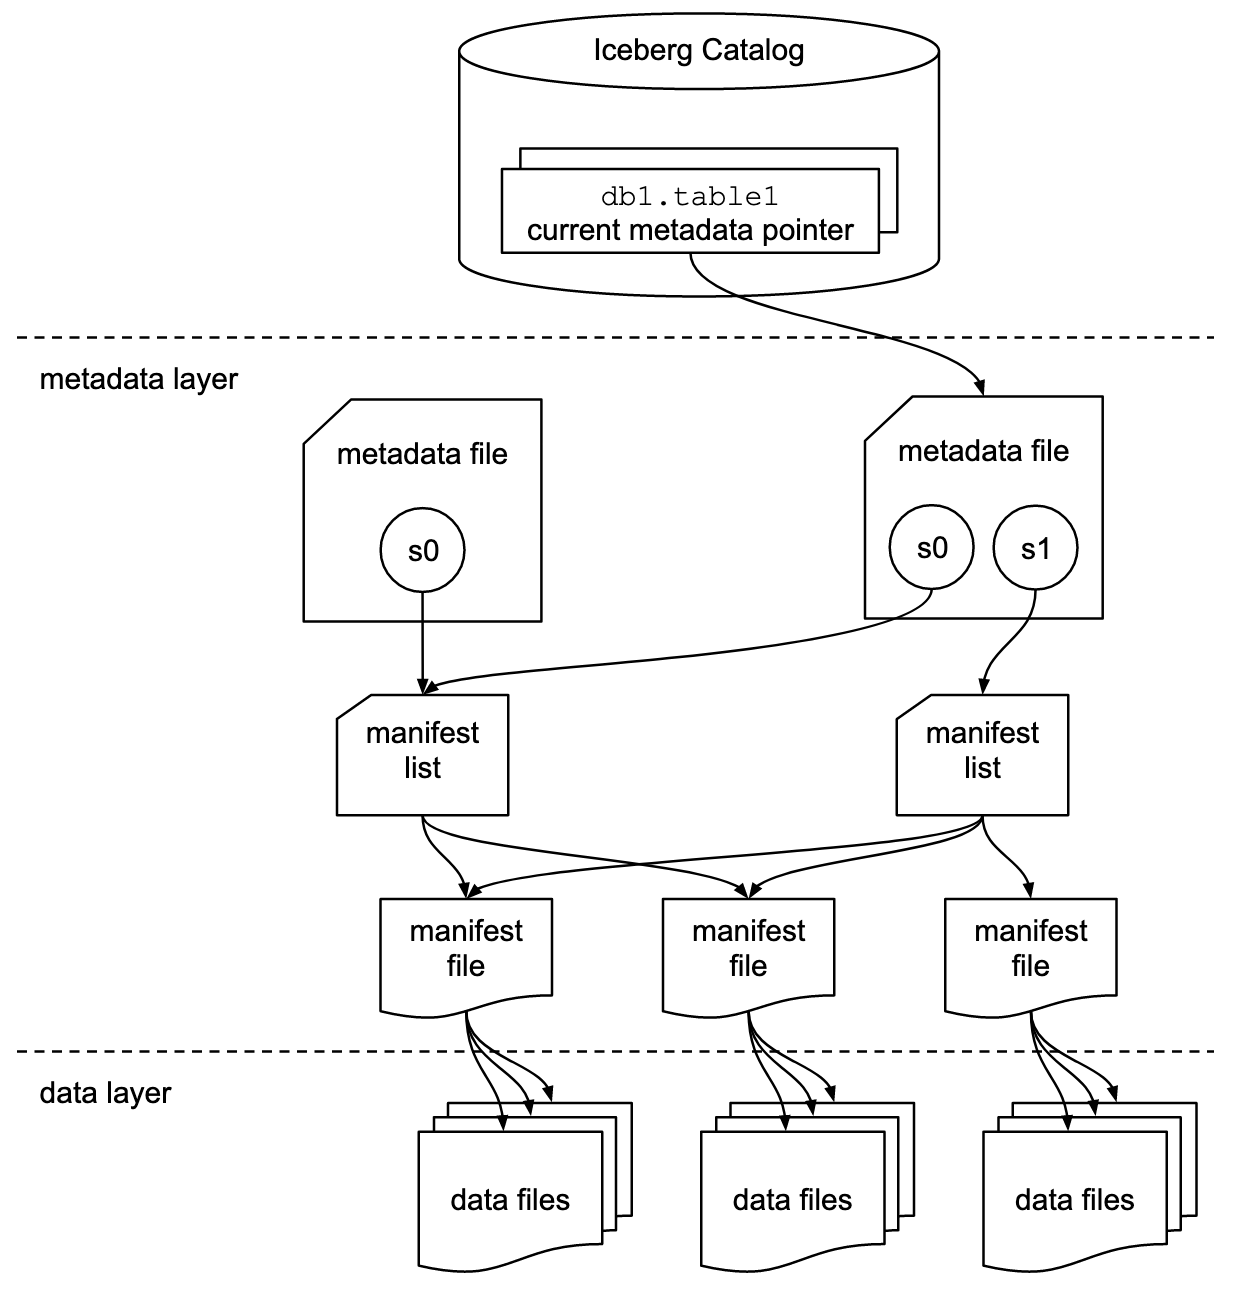
\includegraphics[width=0.8\textwidth]{figuras/iceberg-metadata.png}\\
	\fonte{\cite{iceberg2024}.}
\end{figure}
\FloatBarrier

A Figura \ref{fig:iceberg-metadata} demonstra a estrutura hierárquica de metadados do \textit{Apache Iceberg}, evidenciando como os três níveis principais organizam informações sobre volume, estrutura e distribuição dos dados. Esta organização facilita a extração de metadados relevantes para tomada de decisões de roteamento no \textit{DyraSQL}.

\subsection{Processamento em \textit{clusters}}

A execução de consultas SQL em \textit{data lakes} ocorre tipicamente em \textit{clusters} de processamento com capacidades distintas de memória, paralelismo e tempo máximo de consulta. Consultas leves, com volume reduzido e poucas operações, podem ser atendidas por \textit{clusters} menores, com menor consumo de recursos. Consultas intermediárias demandam paralelismo moderado. Consultas pesadas, com grande volume de dados ou elevada complexidade, requerem \textit{clusters} mais robustos \cite{trinoconcepts,ibmbigdata}.

O \textit{DyraSQL} adota três faixas de capacidade, \textit{cluster small}, \textit{cluster medium} e \textit{cluster large}, implementadas no ambiente local como três instâncias \textit{Trino} com limites distintos de memória e tempo de execução. A classificação em faixas permite que o algoritmo de pontuação selecione o ambiente antes da execução, evitando tanto a subutilização de infraestrutura robusta em consultas simples quanto a saturação de \textit{clusters small} em consultas pesadas.

\subsection{Roteamento Dinâmico de Consultas}

O roteamento dinâmico de consultas envolve a seleção automática do ambiente de execução mais adequado baseado em características da consulta e dos dados, sendo uma abordagem explorada em diversos contextos para melhoria de recursos computacionais. Trabalhos recentes têm demonstrado a importância de execução adaptativa e robusta de consultas em ambientes de \textit{data lakehouse} \cite{xue2024}, sendo que abordagens baseadas em modelos de custo aprendidos \cite{strausz2025} e elasticidade em tempo de execução \cite{zhang2025} têm sido exploradas para melhoria de custo-benefício. O \textit{DyraSQL} implementa roteamento dinâmico baseado em análise prévia de metadados de tabelas \textit{Apache Iceberg}, direcionando consultas para \textit{clusters small}, \textit{medium} ou \textit{large} com base em volume de dados, complexidade da consulta e histórico de execuções similares.


% Inclusão da revisão bibliográfica
\section{Revisão Bibliográfica}
\label{sec:revisao-bibliografica}

Esta seção apresenta uma revisão de trabalhos relacionados ao roteamento dinâmico de consultas, melhoria de custo-benefício em ambientes de processamento e utilização de metadados para tomada de decisões em sistemas de dados. A revisão bibliográfica complementa o referencial teórico apresentado na Seção~\ref{sec:referencial-teorico}, focando em trabalhos que abordam problemas similares ao proposto neste trabalho e técnicas relacionadas utilizadas na literatura.

\subsection{Trabalhos sobre Roteamento Dinâmico de Consultas}

Xue et al. (2024) propuseram um sistema adaptativo que ajusta dinamicamente a estratégia de execução em ambientes de \textit{lakehouse} em larga escala, conforme características da consulta e condições do ambiente \cite{xue2024}; o \textit{DyraSQL} complementa essa abordagem através de análise prévia de metadados antes da execução, em vez de ajustes em tempo real.

Strausz, Pardon e Giurgiu (2025) propuseram um otimizador baseado em modelo de custo aprendido para \textit{workloads} SQL \textit{multi-engine}, prevendo por aprendizado de máquina o custo de execução em diferentes \textit{engines} \cite{strausz2025}; o \textit{DyraSQL} utiliza abordagem similar através do Fator histórico, mas foca em roteamento entre configurações de \textit{clusters Trino}, e não entre \textit{engines} distintas.

Zhang, Zhang e Meng (2025) exploraram elasticidade em tempo de execução, ajustando recursos computacionais durante a execução com base em métricas de \textit{performance} em tempo real \cite{zhang2025}; o \textit{DyraSQL} é complementar, pois realiza a análise prévia de metadados para seleção do \textit{cluster} antes da submissão, e não ajustes durante a execução.

\subsection{Trabalhos sobre Custos em \textit{data lakes}}

Weintraub et al. (2024) propuseram uma abordagem de melhoria de consultas em \textit{data lakes} baseada em planos de cobertura balanceados, utilizando índices e metadados para reduzir o volume de dados via \textit{data skipping} \cite{weintraub2024}; o \textit{DyraSQL} usa abordagem similar de análise de metadados do \textit{Apache Iceberg}, mas para direcionar consultas entre \textit{clusters}, e não para otimizar dentro de uma única arquitetura.

Ding et al. (2024) apresentaram um sistema de \textit{layouts} de dados multidimensionais automatizados no Amazon Redshift, que usa aprendizado de máquina para organizar dados conforme padrões de consultas \cite{ding2024}; o \textit{DyraSQL} utiliza abordagem similar de aprendizado contínuo, ajustando pesos do modelo de decisão a partir do histórico de custo e \textit{performance}, mas com foco em roteamento entre arquiteturas de processamento, e não em organização de dados.

\subsection{Trabalhos sobre Utilização de Metadados}

A utilização de metadados para melhoria de consultas tem sido amplamente explorada na literatura, sendo que sistemas como o \textit{Apache Iceberg} oferecem estruturas hierárquicas de metadados para estimativa de volume, análise de partições e melhoria de consultas \cite{iceberg2024}. Trabalhos anteriores demonstraram a eficácia de metadados para \textit{data skipping} e melhoria de consultas \cite{weintraub2024}; o \textit{DyraSQL} estende essa abordagem para roteamento dinâmico entre diferentes \textit{clusters}.

Sistemas de processamento distribuído como o \textit{Trino} e Apache Spark utilizam metadados para melhoria de planos de execução, sendo que informações sobre volume de dados, distribuição e partições são fundamentais para determinação da estratégia de processamento \cite{trinoconcepts,apachespark2025}. O \textit{DyraSQL} complementa esta abordagem através de utilização de metadados para seleção da arquitetura de processamento antes da geração do plano de execução, sendo que esta análise prévia permite direcionamento mais eficiente das consultas.

\subsection{Diferenças e Contribuições do \textit{DyraSQL}}

O \textit{DyraSQL} diferencia-se dos trabalhos relacionados através de sua abordagem de roteamento dinâmico baseado em análise prévia de metadados do \textit{Apache Iceberg} para direcionamento de consultas entre \textit{clusters} \textit{Trino} de capacidades distintas. Enquanto trabalhos anteriores focam em melhoria dentro de uma única arquitetura \cite{weintraub2024} ou seleção entre diferentes \textit{engines} \cite{strausz2025}, o \textit{DyraSQL} propõe roteamento entre níveis de infraestrutura (\textit{small}, \textit{medium} e \textit{large}) baseado em características de cada consulta identificadas através de metadados.

A principal contribuição do \textit{DyraSQL} reside na combinação de análise prévia de metadados, algoritmo de decisão baseado em pontuação e sistema de histórico para roteamento dinâmico que melhora a relação entre custo e \textit{performance}, complementando trabalhos que focam em melhoria durante a execução \cite{zhang2025} ou seleção entre \textit{engines} \cite{strausz2025} com uma camada adicional de seleção prévia do \textit{cluster}. Os experimentos em ambiente local demonstram que essa abordagem resulta em classificação consistente das consultas.


% Inclusão da metodologia
\section{Metodologia}
\label{sec:metodologia}

A metodologia proposta fundamenta-se na análise sistemática de metadados de tabelas \textit{Apache Iceberg} para tomada de decisões sobre o ambiente de execução mais adequado, resultando em melhor custo-benefício no processamento. O sistema proposto, denominado \textit{DyraSQL}, implementa roteamento dinâmico de consultas SQL baseado em metadados.

\subsection{Arquitetura da Solução Proposta}

O \textit{DyraSQL} implementa uma arquitetura que integra múltiplos componentes para análise de consultas e direcionamento automático para \textit{clusters} com capacidades distintas. A arquitetura é composta por quatro componentes principais que trabalham de forma integrada, direcionando consultas leves para \textit{clusters} menores e consultas pesadas para infraestrutura mais robusta. O \textit{Query Analyzer} executa o comando \textit{EXPLAIN (TYPE IO)} do \textit{Trino} para extrair metadados sobre volume de dados, custos de I/O e características das consultas, incluindo tamanho estimado dos dados de saída, número estimado de linhas, custo de CPU e informações sobre filtros aplicados. O \textit{Decision Engine} aplica o algoritmo de pontuação baseado nos metadados extraídos para determinar o ambiente de execução mais adequado (\textit{small}, \textit{medium} ou \textit{large}). O \textit{Trino Gateway Proxy} intercepta consultas SQL e integra-se com o \textit{DyraSQL Core} para obter decisões de roteamento, direcionando a consulta para o \textit{cluster} selecionado através do \textit{Trino Gateway} oficial. O \textit{Monitoring System} coleta métricas de execução e atualiza o histórico para aprendizado contínuo.

\begin{figure}[ht]
	\centering
	\caption{Contexto do Sistema - DyraSQL}
	\label{fig:contexto-sistema}
	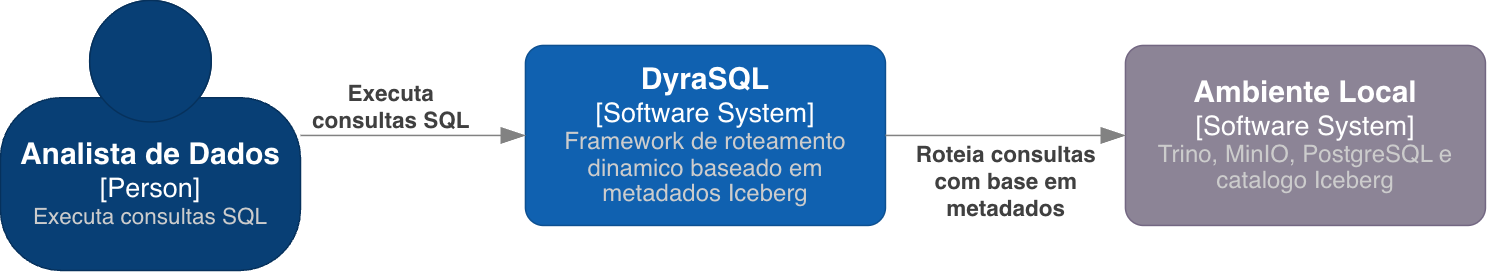
\includegraphics[width=0.9\textwidth]{figuras/contexto.png}\\
	\fonte{Elaborado pelo autor.}
\end{figure}
\FloatBarrier

A Figura \ref{fig:contexto-sistema} apresenta o contexto do \textit{DyraSQL}, mostrando como o sistema se relaciona com usuários e com o ambiente de execução local. O analista de dados executa consultas SQL que são processadas pelo \textit{DyraSQL}, que utiliza \textit{clusters} \textit{Trino} e o \textit{data lake} local para roteamento.

\begin{figure}[ht]
	\centering
	\caption{Containers do Sistema - \textit{DyraSQL}}
	\label{fig:containers-sistema}
	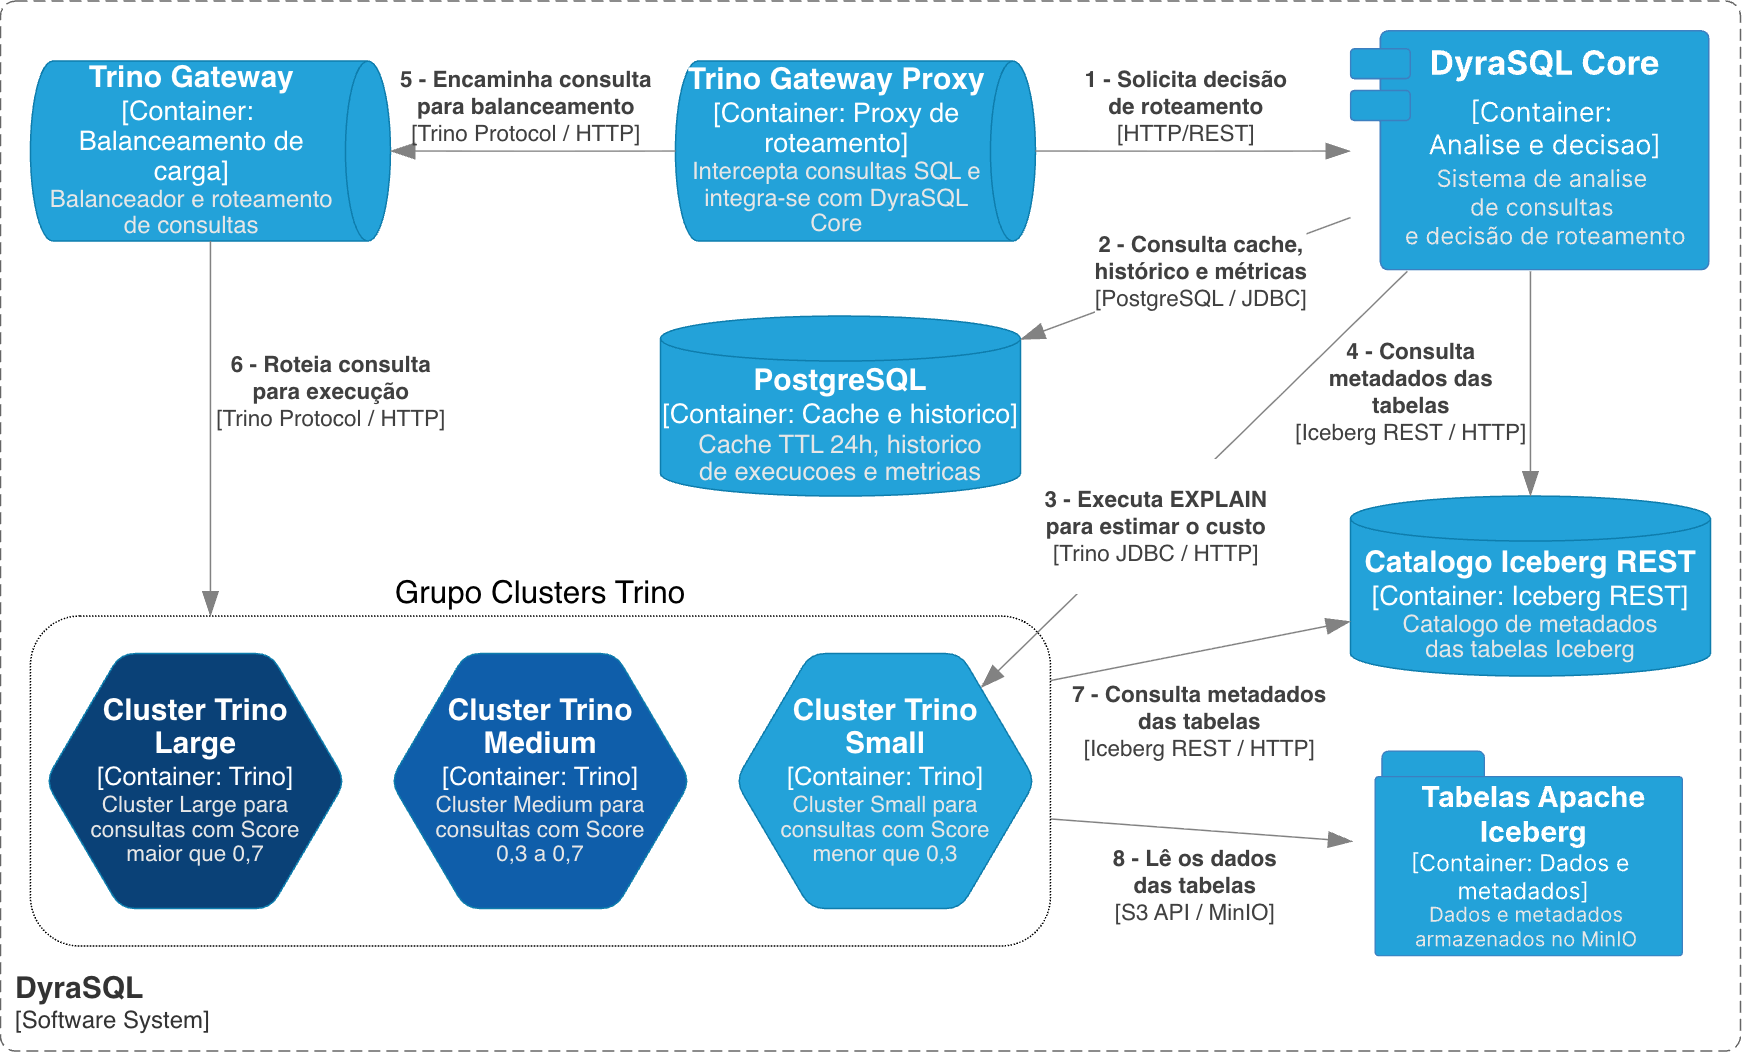
\includegraphics[width=0.9\textwidth]{figuras/container.png}\\
	\fonte{Elaborado pelo autor.}
\end{figure}
\FloatBarrier

A Figura \ref{fig:containers-sistema} detalha a arquitetura de containers do \textit{DyraSQL}, evidenciando os principais componentes, sendo que o \textit{Trino Gateway Proxy} é responsável pela interceptação de consultas e integração com o \textit{DyraSQL Core}, o \textit{Trino Gateway} oficial atua como balanceador, o \textit{DyraSQL Core} realiza a análise de consultas utilizando \textit{EXPLAIN (TYPE IO)} e a decisão de roteamento, e os \textit{clusters} de execução realizam o processamento. A integração com PostgreSQL permite o armazenamento de histórico e \textit{cache} de decisões, enquanto o acesso aos metadados é realizado através do comando \textit{EXPLAIN (TYPE IO)} do \textit{Trino} sobre tabelas no MinIO. Os três \textit{containers Trino} representados na Figura \ref{fig:containers-sistema}, denominados \textit{cluster large}, \textit{cluster medium} e \textit{cluster small}, correspondem às três faixas de capacidade descritas na Seção~\ref{sec:algoritmo-decisao}, sendo cada um configurado com limites distintos de memória e paralelismo dentro do ambiente Docker Compose e acessando igualmente o mesmo Catálogo Iceberg REST, o que garante consistência dos dados independentemente do \textit{container} selecionado.

\begin{figure}[ht]
	\centering
	\caption{Componentes do \textit{DyraSQL} Core}
	\label{fig:componentes-sistema}
	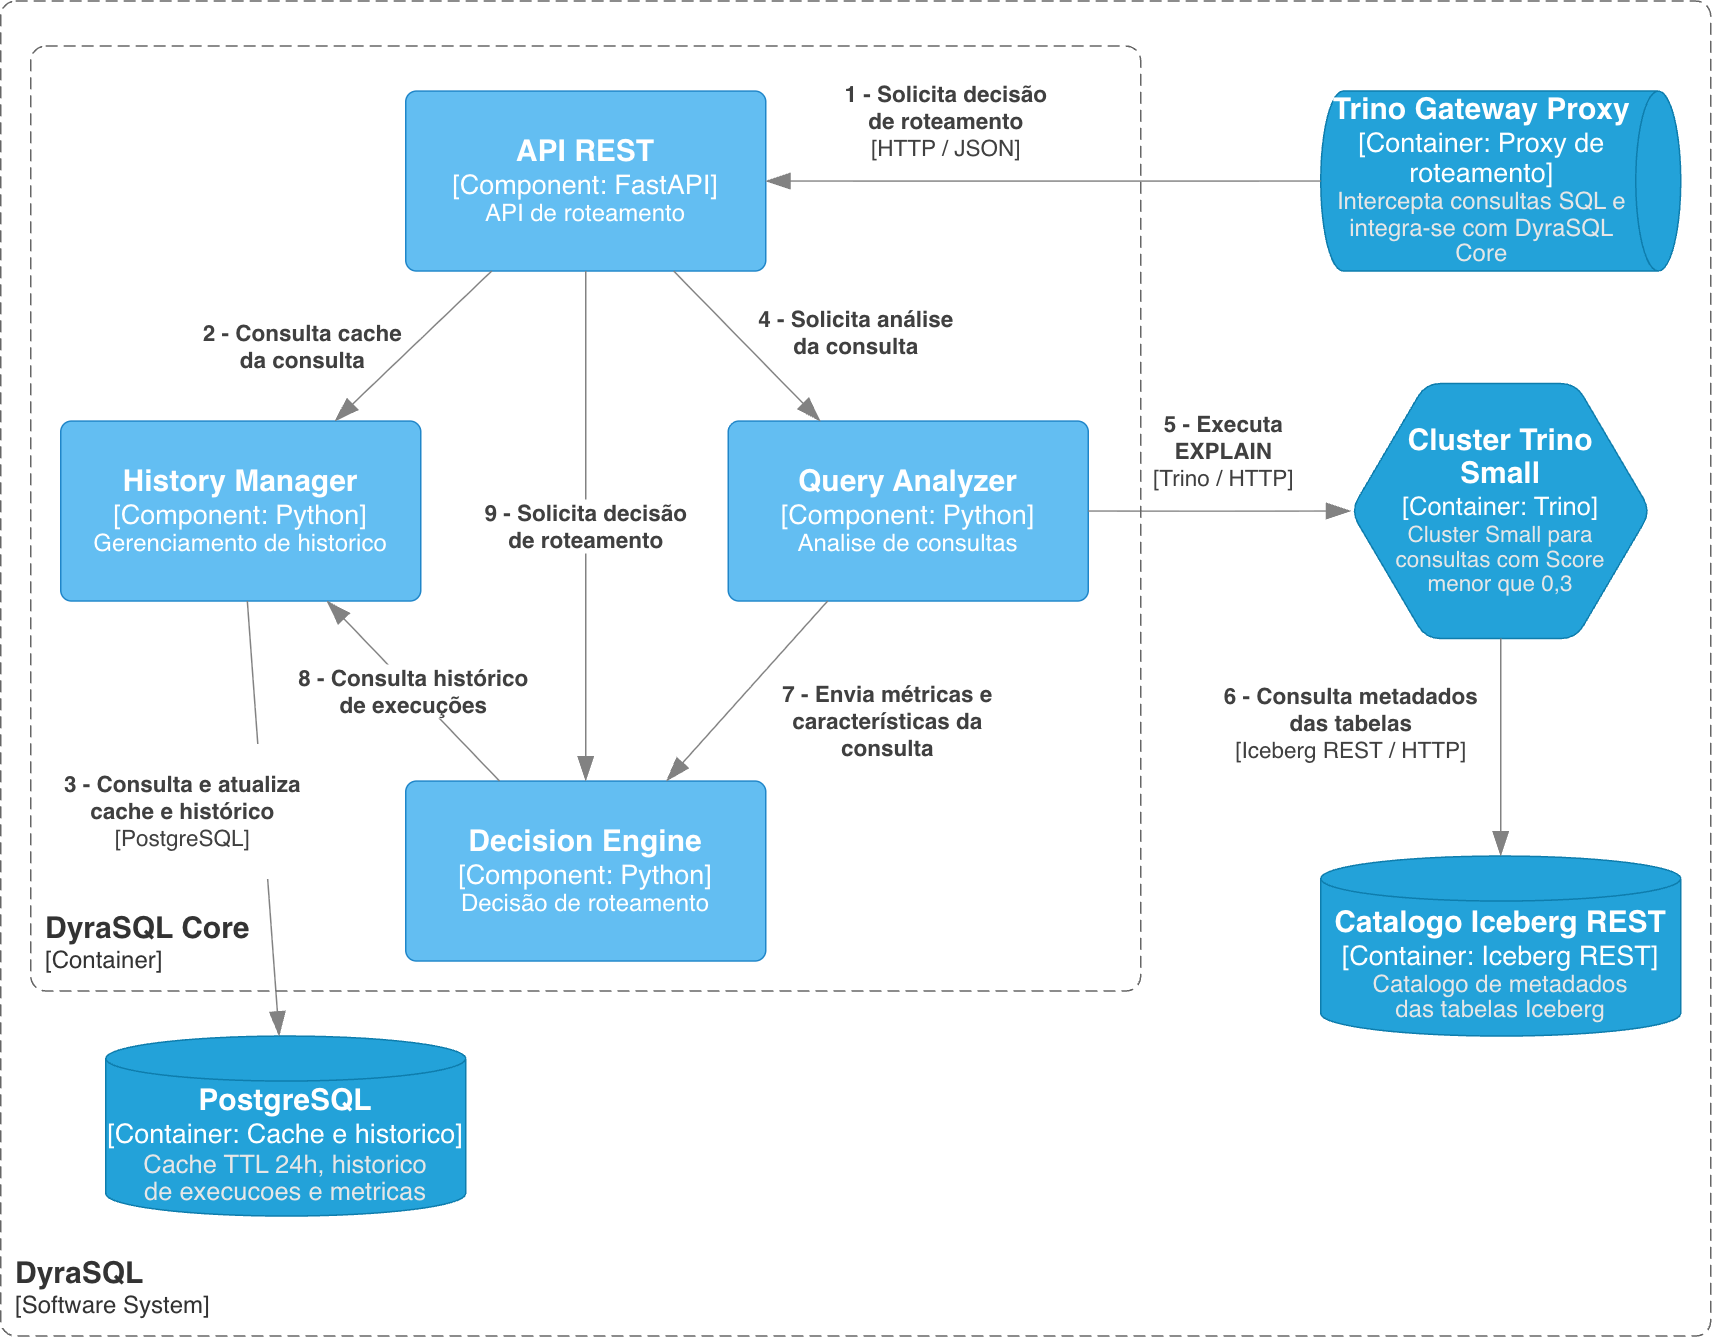
\includegraphics[width=0.9\textwidth]{figuras/componentes.png}\\
	\fonte{Elaborado pelo autor.}
\end{figure}
\FloatBarrier

A Figura \ref{fig:componentes-sistema} apresenta os componentes internos do \textit{DyraSQL Core}, demonstrando o fluxo de dados desde a interceptação da consulta até a execução no \textit{cluster} selecionado e o \textit{feedback} para o histórico. A arquitetura evidencia a integração entre os componentes do sistema, sendo que cada módulo contribui para o processo de tomada de decisão baseado em metadados.

\subsection{Extração de Metadados Relevantes}

O \textit{DyraSQL} utiliza o comando \textit{EXPLAIN (TYPE IO)} do \textit{Trino} para extrair informações sobre o volume de dados e custos de I/O que serão processados por cada consulta SQL. Esta abordagem aproveita a capacidade do \textit{Trino} de analisar consultas antes da execução, fornecendo estimativas baseadas no plano de execução. O \textit{EXPLAIN (TYPE IO)} retorna informações estruturadas em formato \textit{JSON} contendo os metadados necessários para o Algoritmo de decisão, sendo que o sistema extrai especificamente \textit{outputSizeInBytes}, tamanho estimado dos dados de saída em \textit{bytes}, já considerando filtros aplicados; \textit{outputRowCount}, número estimado de linhas; \textit{cpuCost}, custo estimado de processamento; e \textit{columnConstraints}, informações sobre filtros aplicados nas colunas. A Tabela \ref{tab:siglas-calculo} apresenta as siglas utilizadas nos cálculos do Algoritmo de decisão.

\begin{table}[ht]
	\centering
	\caption{Siglas Utilizadas nos Cálculos do Algoritmo de Decisão}
	\label{tab:siglas-calculo}
	\begin{tabular}{ll}
	\hline
	\textbf{Sigla} & \textbf{Descrição} \\
	\hline
	$S$ & \textit{Score} final do Algoritmo de decisão \\
	$f_v$ & Fator de volume normalizado \\
	$f_c$ & Fator de complexidade normalizado \\
	$f_h$ & Fator histórico normalizado \\
	$w_1$ & Peso do Fator volume \\
	$w_2$ & Peso do Fator complexidade \\
	$w_3$ & Peso do Fator histórico \\
	$T_e$ & Tamanho efetivo em GB (obtido de \textit{outputSizeInBytes}) \\
	$R_e$ & Número de linhas efetivas (obtido de \textit{outputRowCount}) \\
	$C_e$ & Custo de CPU efetivo (obtido de \textit{cpuCost}) \\
	$T_{max}$ & Limite máximo de tamanho em GB \\
	$R_{max}$ & Limite máximo de linhas \\
	$F_o$ & Fator de ajuste \\
	$J$ & Número de JOINs \\
	$Ag$ & Número de agregações \\
	$S_q$ & Número de subconsultas \\
	$F_p$ & Número de filtros particionados \\
	$F_{np}$ & Número de filtros não-particionados \\
	$L_c$ & Limite de complexidade \\
	$S_p$ & \textit{Score} prévio da mesma consulta \\
	\hline
	\end{tabular}
	\fonte{Elaborado pelo autor.}
\end{table}
\FloatBarrier

A Tabela \ref{tab:siglas-calculo} apresenta as variáveis utilizadas no Algoritmo de decisão, organizadas desde o \textit{Score} final até os parâmetros específicos de cada fator. Esta padronização uniformiza a notação matemática utilizada nas fórmulas do Algoritmo, facilitando a compreensão dos cálculos nas seções subsequentes. Com essas variáveis definidas, é possível demonstrar a aplicação prática da metodologia através de um exemplo concreto de consulta SQL.

\subsection{Consulta SQL de Referência}

Para demonstrar a aplicação prática da metodologia, considera-se a consulta SQL apresentada no Algoritmo \ref{alg:consulta-vendas}, que processa a Tabela \ref{tab:dataset-teste}. A escolha dessa consulta como referência não é arbitrária, sendo que sua estrutura combina, deliberadamente, um volume de dados moderado, filtro por coluna particionada e complexidade estrutural intermediária, de modo que os três fatores do Algoritmo de decisão, volume, complexidade e histórico, contribuam de forma perceptível para o \textit{Score} final. Consultas mais simples, sem \textit{JOIN} ou agregações, tenderiam a produzir Fator de complexidade próximo de zero, mascarando a contribuição relativa do Fator volume no cálculo, o que motivou a seleção de uma consulta com complexidade intermediária para fins de demonstração.

\begin{table}[ht]
	\centering
	\caption{Dataset de Teste}
	\label{tab:dataset-teste}
	\begin{tabular}{ll}
	\hline
	\textbf{Característica} & \textbf{Descrição} \\
	\hline
	Formato & \textit{Apache Iceberg} \\
	Armazenamento & MinIO \\
	Tamanho aproximado & Até 10 GB \\
	Particionamento & Coluna \textit{date} (função \textit{day}) \\
	Origem & Tabela sintética gerada no ambiente local \\
	\hline
	\textbf{Colunas} & \textbf{Tipo} \\
	\hline
	\textit{tenant\_id} & string \\
	status & string \\
	valor & double \\
	\textit{date} & timestamp \\
	\textit{created\_at} & timestamp \\
	\textit{updated\_at} & timestamp \\
	document & string (\textit{JSON}) \\
	\textit{surrogate\_key} & string \\
	\hline
	\end{tabular}
	\fonte{Elaborado pelo autor.}
\end{table}
\FloatBarrier

A Tabela \ref{tab:dataset-teste} apresenta as características do \textit{dataset} utilizado para demonstração da metodologia proposta, sendo que o formato \textit{Apache Iceberg} permite particionamento por \textit{date}, facilitando a aplicação de filtros que reduzem o volume efetivo de dados processados. O armazenamento no MinIO e o tamanho de até 10 GB representam um cenário controlado para execução local, dimensionado para caber na memória disponível da máquina utilizada nos experimentos, sendo que o particionamento pela função \textit{day} aplicada à coluna \textit{date} permite que o sistema processe apenas frações relevantes dos dados através de filtros temporais. Os registros foram gerados por um script de dados sintéticos, executado continuamente por um período determinado, simulando o crescimento incremental de um \textit{data lake} em produção.

\begin{algorithm}[ht]
\caption{Consulta de Análise de Dados}
\label{alg:consulta-vendas}
\begin{algorithmic}[1]
\REQUIRE Tabela \textit{Apache Iceberg} no MinIO (Tabela \ref{tab:dataset-teste})
\ENSURE Relatório agregado por tenant e período
\STATE SELECT t.tenant\_id, t.categoria, COUNT(*) as total\_registros
\STATE SUM(d.valor) as valor\_total, AVG(d.valor) as valor\_medio
\STATE FROM dados d
\STATE JOIN tenant\_info t ON d.tenant\_id = t.tenant\_id
\STATE WHERE d.date >= '2024-01-01' AND d.date < '2024-02-01'
\STATE AND d.status = 'ATIVO'
\STATE AND t.categoria IN (SELECT categoria FROM tenant\_info WHERE nivel > (SELECT AVG(nivel) FROM tenant\_info))
\STATE GROUP BY t.tenant\_id, t.categoria
\STATE HAVING COUNT(*) > 100
\STATE ORDER BY valor\_total DESC
\STATE LIMIT 50;
\end{algorithmic}
\end{algorithm}
\FloatBarrier

Esta consulta possui 1 JOIN com tabela de dimensão (tenant\_info) utilizando a chave tenant\_id, 3 agregações (COUNT, SUM, AVG), 2 subconsultas e filtros por data e status. O sistema analisa a complexidade estrutural da consulta, identificando operações que requerem processamento distribuído. O filtro por data na coluna particionada permite que o sistema processe apenas uma fração dos dados armazenados, sendo que o \textit{range} da cláusula WHERE determina a quantidade efetiva de dados a serem lidos.

\subsection{Algoritmo de Decisão de Roteamento}
\label{sec:algoritmo-decisao}

O Algoritmo de decisão implementa uma abordagem baseada em pontuação que combina metadados extraídos com características da consulta SQL. O processo opera em duas fases principais, sendo que a primeira é a verificação de \textit{cache}, que consulta o PostgreSQL para verificar se existe uma decisão recente para a mesma \textit{query fingerprint}, e a segunda é o cálculo dinâmico, que executa análise completa dos metadados quando não há \textit{cache} válido. O \textit{fingerprint} é obtido normalizando a consulta SQL original (letras minúsculas, espaços colapsados e literais substituídos por um marcador genérico) e aplicando a função \textit{hash} SHA-256 sobre o resultado, de modo que consultas estruturalmente idênticas com valores de filtro distintos produzam o mesmo \textit{fingerprint} e reaproveitem o \textit{cache}.

O \textit{DyraSQL} mantém um \textit{cache} temporal no PostgreSQL com \textit{TTL} (\textit{Time To Live}) de 24 horas, considerando que o volume de dados pode crescer através de ingestões. Para consultas com \textit{fingerprint} similar executadas nas últimas 24 horas, o sistema recupera diretamente a decisão de roteamento armazenada, eliminando a necessidade de re-análise dos metadados. Quando o \textit{cache} expira ou não existe, o sistema executa o comando \textit{EXPLAIN (TYPE IO)} no \textit{Trino} para obter informações sobre o volume de dados e custos de I/O. O Algoritmo então considera três fatores para determinar a arquitetura mais adequada, sendo que o primeiro é o volume de dados, baseado no campo \textit{outputSizeInBytes} retornado pelo \textit{EXPLAIN (TYPE IO)}, o segundo é a complexidade da consulta, analisando número de JOINs, agregações e subconsultas, e o terceiro é o histórico de execução, utilizando padrões de consultas similares. A Pontuação é calculada através da Equação \ref{eq:pontuacao}.

\begin{equation}
\label{eq:pontuacao}
S = w_1 \times f_v + w_2 \times f_c + w_3 \times f_h
\end{equation}

Com base no \textit{Score} calculado, as consultas são direcionadas para diferentes arquiteturas, sendo que \textit{Scores} menores que 0,3 são direcionados para o \textit{cluster small}, \textit{Scores} entre 0,3 e 0,7 para o \textit{cluster medium}, e \textit{Scores} maiores que 0,7 para o \textit{cluster large}. O sistema pode ajustar os pesos baseado no histórico de custo e \textit{performance} das decisões tomadas, aprendendo qual arquitetura oferece melhor relação entre custo e \textit{performance} para cada tipo de consulta.

\subsubsection{Exemplo Prático de Cálculo}

Para demonstrar o funcionamento do Algoritmo, considera-se o Algoritmo \ref{alg:consulta-vendas} executado sobre a Tabela \ref{tab:dataset-teste}. O sistema executa \textit{EXPLAIN (TYPE IO)} no \textit{Trino}, que retorna informações sobre o volume efetivo de dados a serem processados, já considerando os filtros aplicados. Para este exemplo, o \textit{EXPLAIN (TYPE IO)} retorna \textit{outputSizeInBytes} de aproximadamente 1,25 GB (1.342.177.280 \textit{bytes}) e \textit{outputRowCount} de aproximadamente 2.500.000 linhas, indicando que apenas uma fração dos dados seria processada devido ao filtro por \textit{date} na coluna particionada. No ambiente local o volume absoluto é menor, porém a mesma normalização se aplica, sendo que o exemplo numérico ilustra o cálculo independentemente da escala do \textit{warehouse}.

O Fator volume é calculado através da Equação \ref{eq:fator-volume}, sendo que o sistema utiliza os dados retornados pelo \textit{EXPLAIN (TYPE IO)}, normalizando separadamente o tamanho em GB e o número de linhas usando logaritmos, e combina os valores normalizados com pesos de 0,6 para tamanho e 0,4 para linhas, aplicando um fator de 0,1.

\begin{equation}
\label{eq:fator-volume}
f_v = \left( \frac{\log(T_e)}{\log(T_{max})} \times 0,6 + \frac{\log(R_e)}{\log(R_{max})} \times 0,4 \right) \times (1 - F_o)
\end{equation}

Para o exemplo, o \textit{EXPLAIN (TYPE IO)} retorna tamanho de 1,25 GB ($T_e = 1,25$) e aproximadamente 2.500.000 linhas ($R_e = 2.500.000$), com $T_{max} = 1000$ GB, $R_{max} = 10^9$ e $F_o = 0,1$, resultando em normalização de tamanho de 0,03 e normalização de linhas de 0,71, calculando o Fator volume através da Equação \ref{eq:fator-volume-exemplo}.

\begin{equation}
\label{eq:fator-volume-exemplo}
f_v = \left( \frac{\log(1,25)}{\log(1000)} \times 0,6 + \frac{\log(2500000)}{\log(10^9)} \times 0,4 \right) \times 0,9 = (0,03 \times 0,6 + 0,71 \times 0,4) \times 0,9 = 0,27
\end{equation}

A análise estrutural da consulta é realizada por meio da biblioteca \textit{sqlglot}, que converte o texto SQL em uma árvore de sintaxe abstrata, permitindo identificar precisamente o número de \textit{JOINs}, as agregações da lista de projeção do \textit{SELECT} principal, as subconsultas e os filtros do \textit{WHERE} de nível superior agrupados pela coluna referenciada, evitando ambiguidades de uma análise baseada em expressões regulares (como contabilizar duplamente uma agregação repetida em \textit{HAVING}). Para a consulta do Algoritmo \ref{alg:consulta-vendas}, essa análise identifica 1 JOIN, 3 agregações, 2 subconsultas, 1 filtro particionado e 2 não-particionados. Este cálculo considera a complexidade das operações SQL para determinar o nível de recursos computacionais necessários, sendo calculado através da Equação \ref{eq:fator-complexidade}.

\begin{equation}
\label{eq:fator-complexidade}
f_c = \frac{1 \times 0.2 + 3 \times 0.15 + 2 \times 0.25 + 1 \times 0.02 + 2 \times 0.1}{2.0} = 0.69
\end{equation}

Os coeficientes atribuídos a cada elemento estrutural, como 0,2 por \textit{JOIN} e 0,25 por subconsulta, não derivam de um estudo estatístico sobre custo real de execução, mas são parâmetros configuráveis conforme regras de negócio de cada organização, devendo ser calibrados de acordo com o perfil de \textit{workload} de cada ambiente de implantação.

O Fator histórico é calculado baseado no histórico de execuções anteriores da mesma consulta (mesmo \textit{fingerprint}). Quando não há histórico disponível, o sistema utiliza um valor \textit{default} de $f_h = 0,5$, representando neutralidade na decisão. Quando há histórico, o Fator histórico é determinado conforme a Tabela \ref{tab:fator-historico}, sendo que o sistema verifica se a execução anterior foi bem-sucedida, utilizando o Score prévio ($f_h = S_p$) em caso de sucesso, ou o complemento do Score prévio ($f_h = 1 - S_p$) em caso de falha. Para o exemplo em questão, considerando que não há histórico disponível, o Fator histórico assume o valor \textit{default}. Com pesos ($w_1 = 0.5$, $w_2 = 0.3$, $w_3 = 0.2$), o Score final é calculado através da Equação \ref{eq:score-final}.

\begin{table}[ht]
	\centering
	\caption{Cálculo do Fator Histórico}
	\label{tab:fator-historico}
	\begin{tabular}{ll}
	\hline
	\textbf{Condição} & \textbf{Valor de $f_h$} \\
	\hline
	Sem histórico disponível & $0,5$ \\
	Execução anterior bem-sucedida & $S_p$ \\
	Execução anterior falhou & $1 - S_p$ \\
	\hline
	\end{tabular}
	\fonte{Elaborado pelo autor.}
\end{table}
\FloatBarrier

\begin{equation}
\label{eq:score-final}
S = 0.5 \times 0.27 + 0.3 \times 0.69 + 0.2 \times 0.5 = 0.44
\end{equation}

Com \textit{Score} de 0,44, a consulta é direcionada para o \textit{cluster medium} (faixa 0,3 a 0,7). Os pesos podem ser ajustados com base no histórico de custo e \textit{performance} das decisões, inspirado em sistemas como o Amazon Redshift MDDL \cite{ding2024}. O Algoritmo principal do \textit{DyraSQL} pode ser expresso através do pseudocódigo apresentado no Algoritmo \ref{alg:roteamento-dinamico}, sendo que este processo garante que cada consulta seja direcionada para o ambiente mais adequado baseado na análise dos metadados obtidos através do \textit{EXPLAIN (TYPE IO)} do \textit{Trino}.

\begin{algorithm}[ht]
\caption{Algoritmo de Roteamento Dinâmico de Consultas}
\label{alg:roteamento-dinamico}
\begin{algorithmic}[1]
\REQUIRE consulta SQL, acesso ao \textit{Trino} para \textit{EXPLAIN (TYPE IO)}, histórico PostgreSQL
\ENSURE cluster selecionado, score calculado
    \STATE Gerar \textit{fingerprint} único da consulta SQL
    \STATE Consultar \textit{cache} no PostgreSQL usando o \textit{fingerprint}
    \STATE \textbf{Se} decisão existe no \textit{cache} \textbf{e} TTL é válido \textbf{então}
    \STATE \quad \textbf{Retornar} cluster armazenado no \textit{cache}
    \STATE \textbf{Fim se}
    \STATE Executar \textit{EXPLAIN (TYPE IO)} no \textit{Trino} para obter metadados
    \STATE Extrair \textit{outputSizeInBytes}, \textit{outputRowCount} e \textit{columnConstraints}
    \STATE Normalizar fator de volume baseado em \textit{outputSizeInBytes}
    \STATE Analisar complexidade da consulta SQL
    \STATE Consultar histórico de consultas similares
    \STATE Calcular score usando fórmula ponderada
    \STATE \textbf{Se} score é menor que 0,3 \textbf{então}
    \STATE \quad Selecionar cluster small
    \STATE \textbf{Senão se} score está entre 0,3 e 0,7 \textbf{então}
    \STATE \quad Selecionar cluster medium
    \STATE \textbf{Senão}
    \STATE \quad Selecionar cluster large
    \STATE \textbf{Fim se}
    \STATE Salvar decisão no histórico do PostgreSQL
    \STATE \textbf{Retornar} cluster selecionado
\end{algorithmic}
\end{algorithm}
\FloatBarrier

O pseudocódigo demonstra o fluxo completo do Algoritmo, desde a interceptação da consulta até a decisão final de roteamento, incluindo verificação de \textit{cache}, execução do \textit{EXPLAIN (TYPE IO)} para extração de metadados, cálculo do \textit{Score} e seleção do \textit{cluster} apropriado.

\subsection{Sistema de Histórico e Aprendizado}

O \textit{DyraSQL} mantém um histórico de execuções no PostgreSQL, armazenando \textit{fingerprints} de consultas, métricas de custo-benefício e decisões de roteamento. A cada execução de consulta, o sistema pode coletar métricas pós-execução incluindo tempo de execução, custo operacional e eficácia da decisão, salvando essas informações para enriquecimento do histórico. A eficácia é avaliada pela comparação entre o tempo observado e o esperado para a faixa de capacidade, sendo que decisões recorrentemente inadequadas podem indicar a necessidade de ajuste dos pesos $w_1$, $w_2$ e $w_3$ da Equação \ref{eq:pontuacao}.

\subsubsection{Cálculo do Fator Histórico}

O Fator histórico é calculado através da análise do histórico de execuções anteriores da mesma consulta, identificada pelo \textit{fingerprint} único gerado a partir da estrutura da consulta SQL. O sistema consulta o PostgreSQL para verificar se existe uma execução anterior da mesma consulta, sendo que quando não há histórico disponível, o sistema utiliza um valor \textit{default} de $f_h = 0,5$, representando neutralidade na decisão.

Quando há histórico disponível, o sistema verifica se a execução anterior foi bem-sucedida. Se a execução anterior foi bem-sucedida, o Fator histórico utiliza o Score prévio calculado para a mesma consulta ($f_h = S_p$). Se a execução anterior falhou, o Fator histórico utiliza o complemento do Score prévio ($f_h = 1 - S_p$), indicando que a decisão anterior não foi adequada e sugerindo uma arquitetura alternativa.

O Fator histórico é então determinado conforme a Tabela \ref{tab:fator-historico}, sendo que esta abordagem permite que o sistema aprenda com execuções anteriores da mesma consulta. Esta abordagem é inspirada em mecanismos de \textit{learned cost models} implementados em sistemas como o Amazon Redshift \cite{ding2024}. O sistema mantém um \textit{cache} temporal no PostgreSQL com \textit{TTL} de 24 horas, sendo que consultas com \textit{fingerprint} similar executadas nas últimas 24 horas recuperam diretamente a decisão de roteamento armazenada.

\subsection{Integração com \textit{Trino Gateway}}

A solução integra-se ao \textit{Trino} Gateway oficial através de uma arquitetura modular composta por três componentes principais. O primeiro componente é o \textit{Trino} Gateway oficial, compilado a partir do código-fonte em Java, que atua como balanceador e \textit{gateway} de roteamento, utilizando PostgreSQL para persistência de configurações e histórico de \textit{backends}. O segundo componente é o \textit{Trino Gateway Proxy}, desenvolvido em Python utilizando FastAPI, que intercepta consultas SQL antes do roteamento e integra-se com o \textit{DyraSQL Core} para obter decisões baseadas em análise de metadados. O terceiro componente é o \textit{DyraSQL Core}, que implementa o Algoritmo de decisão e fornece a API REST para análise de consultas e cálculo de \textit{scores}. O \textit{Trino Gateway Proxy} consulta o \textit{DyraSQL Core} através do \textit{endpoint} POST /api/v1/route para cada consulta recebida, obtendo a decisão de roteamento com \textit{cluster} recomendado, \textit{score} calculado e fatores utilizados, e então direciona a consulta para o \textit{cluster Trino} apropriado. Esta arquitetura modular permite integração com o \textit{Trino} Gateway oficial sem necessidade de modificações no código-fonte do \textit{gateway}.

O contrato do \textit{endpoint} POST /api/v1/route recebe um objeto \textit{JSON} com a consulta SQL e retorna a decisão de roteamento (\textit{cluster}, \textit{score} e fatores utilizados), conforme exemplo de requisição e resposta apresentado no Apêndice A.

\subsection{Implementação do \textit{framework}}

O \textit{framework DyraSQL} foi desenvolvido utilizando Python para os módulos de roteamento e análise de metadados, Docker Compose para orquestração do ambiente local, e \textit{Trino} como \textit{engine} de consultas. A arquitetura inclui o \textit{Trino Gateway} oficial, o \textit{Trino Gateway Proxy} em FastAPI, PostgreSQL para persistência do \textit{gateway} e para \textit{cache} de decisões, MinIO para armazenamento de objetos das tabelas \textit{Iceberg}, e catálogo REST compartilhado pelos \textit{clusters}.

A configuração do \textit{Trino} utiliza o conector \textit{Iceberg} com catálogo REST e \textit{filesystem} de objetos apontando para o MinIO. Esta configuração garante que os três \textit{clusters} compartilhem o mesmo catálogo de metadados, permitindo acesso unificado às tabelas independentemente do \textit{cluster} de execução. A implementação em Python contempla módulos para análise de consultas SQL utilizando \textit{EXPLAIN (TYPE IO)}, aplicação do Algoritmo de decisão baseado em \textit{scores}, gerenciamento de histórico no PostgreSQL e API REST para integração com o \textit{Trino Gateway Proxy}. O \textit{framework} foi avaliado através de testes com tabelas \textit{Apache Iceberg} geradas no ambiente local, confirmando que o sistema é capaz de calcular \textit{scores} e direcionar consultas para os \textit{clusters} apropriados. O código-fonte completo do protótipo está disponível em repositório público \cite{dyrasql2026}.


% Inclusão dos experimentos e resultados
\section{Experimentos e Resultados}
\label{sec:experimentos}

Esta seção apresenta o ambiente empregado para avaliação do \textit{framework DyraSQL}, os cenários de teste, as métricas observadas e a discussão dos resultados. Os experimentos foram projetados para verificar a consistência da lógica de roteamento e dos pesos do Algoritmo de decisão em ambiente local, confirmando que o sistema calcula \textit{scores} e classifica consultas nas faixas de capacidade definidas.

\subsection{Ambiente de Teste}

Os experimentos foram conduzidos em ambiente local orquestrado por Docker Compose, com tabelas \textit{Apache Iceberg} geradas sobre o MinIO e catálogo REST compartilhado pelos \textit{clusters} \textit{Trino}. A Tabela \ref{tab:dataset-teste} foi utilizada como caso de referência, sendo que a consulta principal foi apresentada através do Algoritmo \ref{alg:consulta-vendas}. Experimentos adicionais variaram o \textit{range} de filtros por data para processar diferentes volumes efetivos.

A Tabela \ref{tab:ambiente-teste} apresenta as configurações do ambiente de teste. O \textit{framework} direciona consultas para três \textit{clusters} baseado no \textit{Score} calculado, sendo que consultas com \textit{Score} menor que 0,3 seguem para o \textit{cluster small}, consultas com \textit{Score} entre 0,3 e 0,7 para o \textit{cluster medium}, e consultas com \textit{Score} maior que 0,7 para o \textit{cluster large}.

\begin{table}[ht]
	\centering
	\caption{Configurações do Ambiente de Teste}
	\label{tab:ambiente-teste}
	\begin{tabular}{lll}
	\hline
	\textbf{Componente} & \textbf{Tipo} & \textbf{Configuração} \\
	\hline
	\textit{cluster small} & \textit{Small} & \textit{Score} menor que 0,3 \\
	\textit{cluster medium} & \textit{Medium} & \textit{Score} 0,3 a 0,7 \\
	\textit{cluster large} & \textit{Large} & \textit{Score} maior que 0,7 \\
	\textit{Trino Gateway} & \textit{gateway} & Balanceador e roteamento \\
	\textit{Trino Gateway Proxy} & \textit{proxy} & Integração com o \textit{DyraSQL Core} \\
	\textit{DyraSQL Core} & API REST & Análise e decisão de roteamento \\
	PostgreSQL & Banco de dados & Persistência do \textit{gateway} e \textit{cache} \\
	MinIO & Objetos & \textit{Warehouse} das tabelas \textit{Iceberg} \\
	Catálogo REST & Catálogo & Metadados das tabelas \textit{Iceberg} \\
	\hline
	\end{tabular}
	\fonte{Elaborado pelo autor.}
\end{table}
\FloatBarrier

A Tabela \ref{tab:ambiente-teste} reúne os componentes da stack local, evidenciando a separação entre decisão de roteamento, catálogo, armazenamento e execução. Os três \textit{clusters} \textit{Trino} compartilham o mesmo catálogo REST e o mesmo \textit{warehouse} no MinIO, de modo que a escolha do destino altera apenas a capacidade de processamento.

\subsection{Cenários de Teste}

Os testes utilizaram a Tabela \ref{tab:dataset-teste} e a consulta do Algoritmo \ref{alg:consulta-vendas}, além de variações com filtros de data mais estreitos ou mais amplos e de consultas apenas de metadados. Os cenários cobriram \textit{cache miss}, primeira execução com cálculo completo do \textit{Score}, e \textit{cache hit}, reexecução com o mesmo \textit{fingerprint} dentro do \textit{TTL} de 24 horas. Também foram observadas consultas de baixa complexidade, encaminhadas ao \textit{cluster small}, e a consulta de referência, cujo exemplo de cálculo resulta em \textit{Score} 0,44 e destino \textit{medium}.

\subsection{Métricas e Resultados}

As métricas observadas incluem consistência dos \textit{scores} para consultas similares, adequação das faixas 0,3 e 0,7, tempo de cálculo associado ao \textit{EXPLAIN (TYPE IO)} e taxa de \textit{cache hit} no PostgreSQL. O \textit{EXPLAIN (TYPE IO)} retornou estimativas de volume e de linhas compatíveis com os filtros de partição aplicados, permitindo o cálculo do Fator volume. A consulta de referência produziu \textit{Score} 0,44, classificada no \textit{cluster medium}, enquanto consultas sem junções e com filtros estreitos tenderam ao \textit{cluster small}. Reexecuções com o mesmo \textit{fingerprint} recuperaram a decisão armazenada, evitando nova análise enquanto o \textit{TTL} permaneceu válido.

Os pesos $w_1 = 0,5$, $w_2 = 0,3$ e $w_3 = 0,2$ diferenciaram consultas leves, intermediárias e pesadas no conjunto avaliado, sendo o fator de volume o de maior influência e o fator histórico complementar quando havia execução prévia. O tempo de análise prévia manteve-se adequado para o \textit{dataset} sintético, permanecendo na ordem de centenas de milissegundos nas consultas observadas.

\subsection{Limitações Identificadas}

O \textit{dataset} sintético possui volume inferior ao de ambientes de produção, o que restringe a generalização dos resultados para \textit{warehouses} de centenas de gigabytes. A precisão das decisões depende de histórico suficiente no PostgreSQL, sendo que consultas novas utilizam $f_h = 0,5$. O \textit{EXPLAIN (TYPE IO)} pode se tornar mais lento em planos muito complexos, e metadados \textit{Iceberg} desatualizados reduzem a qualidade das estimativas. A máquina local também não reproduz elasticidade nem escala de um ambiente de nuvem, aspecto tratado nos trabalhos futuros. O sistema ainda não implementa uma estratégia formal de \textit{fallback} para os casos em que o \textit{EXPLAIN (TYPE IO)} não retorna resultado (indisponibilidade do \textit{Trino} ou \textit{timeout}), resultando em erro em vez de um \textit{cluster} padrão; essa condição não se manifestou nos testes, mas não é coberta pela lógica atual.


% Inclusão das conclusões
\section{Considerações Finais}
\label{sec:consideracoes-finais}
\label{sec:con}

Este trabalho apresentou o desenvolvimento do \textit{DyraSQL}, um mecanismo de decisão para roteamento dinâmico de consultas SQL baseado em metadados de tabelas \textit{Apache Iceberg}. O problema abordado consistiu na necessidade de arquiteturas que se adaptem ao tipo de consulta, evitando provisionamento excessivo de infraestrutura robusta para consultas leves e garantindo recursos adequados para consultas pesadas, resultando em melhor custo-benefício no processamento.

Os objetivos propostos foram alcançados através da análise de metadados \textit{Apache Iceberg}, estabelecimento de regras de decisão para roteamento, desenvolvimento de um \textit{framework} funcional em ambiente local e avaliação da lógica de roteamento. A metodologia envolveu análise dos metadados disponíveis, definição de critérios baseados em volume de dados, complexidade da consulta e histórico de execuções, e verificação da lógica proposta através de testes com tabelas \textit{Iceberg} geradas localmente.

Os principais resultados demonstraram que a lógica de roteamento funciona de forma consistente, sendo que o \textit{framework} é capaz de calcular \textit{scores} e direcionar consultas para os \textit{clusters} apropriados baseado nas características dos dados e na complexidade das consultas. A análise dos metadados revelou informações sobre volume de dados e complexidade que podem ser utilizadas para determinar a arquitetura mais adequada, sendo que o uso do \textit{EXPLAIN (TYPE IO)} do \textit{Trino} fornece estimativas suficientes para o Algoritmo de decisão. A avaliação confirmou que os pesos do Algoritmo funcionam de forma adequada, sendo que a combinação dos fatores de volume, complexidade e histórico resulta em \textit{scores} que diferenciam consultas leves, intermediárias e pesadas.

As contribuições deste trabalho incluem um \textit{framework} para análise de metadados \textit{Apache Iceberg} para determinação de arquiteturas dinâmicas baseado em volume de dados, complexidade de consultas e histórico de execuções; regras de decisão para roteamento automático através de algoritmo de pontuação que combina múltiplos fatores; um protótipo funcional integrando \textit{Trino}, catálogo \textit{Iceberg} REST, MinIO e PostgreSQL, que direciona consultas para \textit{clusters small}, \textit{medium} ou \textit{large}; e a avaliação da lógica de roteamento através de testes com dados sintéticos em ambiente local.

Como limitações do estudo, destacam-se o uso de \textit{dataset} sintético em escala inferior à de produção e a dependência de histórico suficiente no PostgreSQL, sendo que consultas sem histórico apresentam maior probabilidade de decisões menos precisas. A extração de metadados apresenta limitações para consultas muito complexas, sendo que o tempo do \textit{EXPLAIN (TYPE IO)} pode impactar a latência total. O sistema também depende da qualidade dos metadados do \textit{Apache Iceberg}, sendo que tabelas com metadados desatualizados podem resultar em estimativas imprecisas do volume efetivo.

\subsection{Trabalhos Futuros}

Trabalhos futuros concentram-se na aplicação do \textit{DyraSQL} em ambientes de nuvem. O núcleo do sistema, composto pelo cálculo do \textit{Score}, pelo \textit{Trino Gateway} e pelas três faixas de \textit{cluster}, permanece o mesmo, sendo que o que se altera é a implantação. \textit{Clusters} gerenciados em nuvem, por exemplo EMR \cite{awsemr2025}, e o armazenamento de objetos do provedor substituiriam o MinIO e as instâncias \textit{Trino} locais, permitindo avaliar o roteamento com volumes de produção e com elasticidade típica de plataformas gerenciadas.

Outra direção consiste em substituir os pesos $w_1$, $w_2$ e $w_3$, atualmente fixos, por um modelo de aprendizado supervisionado treinado sobre o histórico acumulado no PostgreSQL, de forma similar ao Amazon Redshift MDDL \cite{ding2024}, além de avaliar o \textit{DyraSQL} sobre tabelas de centenas de gigabytes a terabytes, verificando se as faixas de \textit{score} permanecem adequadas em escala real.

Uma limitação da arquitetura atual é que os três \textit{clusters} são \textit{containers} persistentes com capacidade fixa, de modo que um pico de consultas concorrentes na mesma faixa de \textit{score} pode esgotar o \textit{cluster} de destino mesmo com os demais subutilizados. Um trabalho futuro é migrar para um modelo orientado a \textit{tasks}, análogo à distinção que o Amazon ECS estabelece entre \textit{services} de longa duração e \textit{tasks} avulsas sob demanda \cite{awsecs2025}, dimensionando o ambiente de execução individualmente por consulta em vez de compartilhar um \textit{cluster} fixo. Também é necessário definir uma estratégia de \textit{fallback} para os casos em que a análise de metadados não é concluída (indisponibilidade do \textit{Trino} ou \textit{timeout}), direcionando a um \textit{cluster} padrão em vez de retornar erro ao cliente — situação não observada nos testes, mas esperada antes de uma implantação em produção.


%%%%%%%%%%%%%%%%%%%%%%%%%%%%%%%%%%%
%% FIM DO TEXTO
%%%%%%%%%%%%%%%%%%%%%%%%%%%%%%%%%%%

%%%%%%%%%%%%%%%%%%%%%%%%%%%%%%%%%%%
%% Inicio bibliografia
%%%%%%%%%%%%%%%%%%%%%%%%%%%%%%%%%%%

\newpage

\bibliographystyle{abntex2-alf}
\bibliography{bibliografia}

%%%%%%%%%%%%%%%%%%%%%%%%%%%%%%%%%%%
%% Apêndice
%%%%%%%%%%%%%%%%%%%%%%%%%%%%%%%%%%%

\newpage

\begin{center}
\textbf{APÊNDICE A - EXEMPLO DE REQUISIÇÃO E RESPOSTA DA API DE ROTEAMENTO}
\end{center}

\vspace{0.5cm}

Os trechos a seguir ilustram um exemplo de requisição e de resposta do \textit{endpoint} POST /api/v1/route do \textit{DyraSQL Core}, descrito na Seção~\ref{sec:metodologia}.

\begin{center}
\textbf{Quadro 1 - Requisição do \textit{endpoint} POST /api/v1/route}
\end{center}

\begin{framed}
\begin{verbatim}
{
  "query": "SELECT ... FROM dados d JOIN tenant_info t ..."
}
\end{verbatim}
\end{framed}

\fonte{Elaborado pelo autor.}

\vspace{0.8cm}

\begin{center}
\textbf{Quadro 2 - Resposta do \textit{endpoint} POST /api/v1/route}
\end{center}

\begin{framed}
\begin{verbatim}
{
  "fingerprint": "3f2a1c...",
  "cluster": "medium",
  "score": 0.44,
  "factors": {
    "volume": 0.27,
    "complexity": 0.69,
    "historical": 0.5
  },
  "cached": false,
  "cluster_url": "http://trino-medium:8080"
}
\end{verbatim}
\end{framed}

\fonte{Elaborado pelo autor.}


\end{document}